\chapter{Prototyping in Office Message System}
%Introduction
This prototype exemplifies the use of Java RMI Clients and Servers. As well as showing the basics of Remote Method Invocation, a basic leader-election algorithm is implemented. This leader-election takes place if it is discovered, that the current leader has gone down.

In the prototype the leader, and only the leader, will register the function "GloriousLeader" on the RMI Registry. 
If the leader goes down, a new leader will be elected this will ReBind its own GloriousLeader function.

In perspective, the GloriousLeader function should access something that required a single-node access. In this basic prototype, the function returns the NodeID of the leader node as well as short message (as a String object).

\section{System setup}
\subsection{Setting up RMI Registry}
The host machine must host the RMI registry, the service in charge of serving up Remote Method calls.
The RMI Registry uses the CLASSPATH variable to identify the Java classes/methods bound and requested from the host. 

Therefore, the CLASSPATH variable must be set:

\begin{center}
	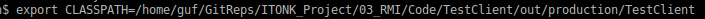
\includegraphics[width=\textwidth]{ExportingClasspath.png}
	\captionof{figure}{Exporting the CLASSPATH variable on Linux}
\end{center}

This is the path to the base directory of the .class files, compiled with the Java Compiler (Through IntelliJ).

When this is done, the RMI registry is started by the command:

\textit{rmiregistry \&}

\subsection{Running the Servers}
When starting the main programs, java needs to know the path to the .class files of the project. The java.rmi.server also needs to know the path to the actual .class files.

This is done through:
[INSERT PICTURE OF STARTING MAIN PROGRAMS]

\section{System description}
The system consists of nodes in a ring-like configuration.

Each node can be either a leader or a slave Node. 
\subsection{Node}
The node is the main entity in the system. Each node has the capacity for being both leader and slave. 

All nodes has a Server and a Client object. After a leader election, if a declares itself the leader, it will create a LeaderClass object for itself. 

\subsubsection{Server}

\subsubsection{Client}

\subsubsection{LeaderClass}

\subsection{System}
\section{Leader Election}
\subsection{Purpose}
\subsection{GloriousLeader function}
\subsection{QuestFunction}

\begin{center}
	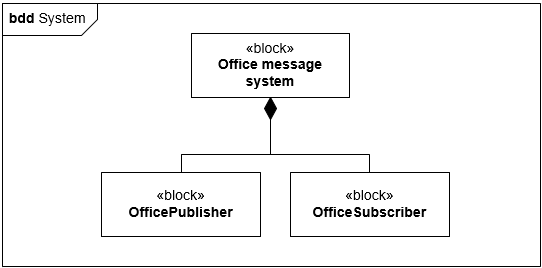
\includegraphics[width=\textwidth]{bdd_image.png}
	\captionof{figure}{BDD of the Office Message System}
\end{center}
\section{Tests}